\documentclass[conference]{IEEEtran}
\IEEEoverridecommandlockouts

\usepackage{cite}
\usepackage{amsmath,amssymb}
\usepackage{graphicx}
\usepackage{booktabs}
\usepackage{url}
\usepackage{tikz}
\usetikzlibrary{arrows.meta}

\begin{document}

\title{LLMSheriff: A Hybrid Framework for Intent-State Inference in Autonomous AI Agents}

\author{
\IEEEauthorblockN{Rajendra Kumar Shaw}
\IEEEauthorblockA{
Kolkata, India \\
rajendra250601@gmail.com
}
}

\maketitle

% -----------------------------------------------------------------------
\begin{abstract}
Autonomous AI agents increasingly execute long-running workflows where failures are not
always explicit. Existing observability platforms capture execution traces but generally
do not infer whether an agent is still making meaningful progress toward its assigned
goal. This paper presents LLMSheriff, an exploratory research prototype that investigates
hybrid intent-state inference from agent execution traces. The system maps low-level
events to eight behavioral states---Planning, Executing, Waiting, Recovering, Stalled,
Abandoned, Completed, and Failed---using a rule-based analyzer and an LLM behavioral analyzer in
parallel. Agreement between analyzers is treated as a confidence signal; disagreement
is surfaced as a diagnostic output rather than suppressed. A behavior interpretation
layer produces evidence summaries, confidence estimates, disagreement explanations,
and human-intervention recommendations.
We evaluate the rule-based analyzer on a corpus of 100 synthetic labelled traces and
report 71\% accuracy and 0.732 macro-F1, with strong performance on unambiguous cases
and systematic errors on waiting and borderline traces. The work is exploratory; it
does not claim to solve intent monitoring, but demonstrates one reproducible approach
to behavioral inference above conventional observability.
\end{abstract}

\begin{IEEEkeywords}
agentic AI, execution monitoring, intent inference, goal satisfaction, behavioral observability
\end{IEEEkeywords}

% -----------------------------------------------------------------------
\section{Introduction}

Autonomous AI agents now orchestrate multi-step workflows involving tool calls, retries,
external dependencies, and long idle periods. Standard observability outputs---logs,
latency metrics, retry counts, and exit codes---record \emph{what} happened during
execution. They rarely answer whether the agent is still intentionally pursuing its
assigned goal.

This distinction matters in practice. An agent may run without errors while making no
forward progress: repeating the same search, polling indefinitely, or drifting after an
early failure. Conversely, an agent may encounter setbacks and still recover by adopting
a new strategy. A monitoring layer that only detects hard failures cannot separate these
cases.

LLMSheriff is a research prototype built to explore this gap. It asks:

\begin{quote}
\emph{Can execution traces be interpreted to infer higher-level behavioral states that
help a human decide whether to wait, intervene, or declare success?}
\end{quote}

The contribution is not a production monitoring platform. Rather, we investigate whether
hybrid symbolic and LLM-based inference can produce explainable behavioral states from
traces. A key design choice is that LLMSheriff does not attempt to infer an agent's true
internal intentions. Instead, it infers \emph{behavioral intent} from externally
observable execution traces---a weaker but tractable formulation. When both analyzers
agree, agreement is treated as a confidence signal. When they disagree, the disagreement
itself is surfaced as a diagnostic output, identifying traces where semantic ambiguity
requires human judgement.

% -----------------------------------------------------------------------
\section{Background and Related Work}

\subsection{AI Observability and Agent Monitoring}

Platforms such as LangSmith~\cite{langsmith}, Langfuse~\cite{langfuse}, and AgentOps
provide trace storage, latency analysis, token accounting, and debugging views for LLM
applications. OpenTelemetry~\cite{otel} standardises distributed tracing across
services. These tools excel at reconstructing execution paths and surfacing failures.
They do not, by default, infer goal-level behavioral intent.

Recent work on LLM agent oversight focuses on detecting unsafe tool calls, hallucinated
actions, and policy violations during execution. LLMSheriff differs by targeting
\emph{progress semantics}: whether execution still appears goal-directed rather than
merely error-free. This is a softer but practically important property---an agent that
loops safely is still failing its user.

\subsection{Goal and Plan Recognition}

Goal-oriented requirements engineering treats systems in terms of goals to be achieved
and obstacles to satisfaction~\cite{horkoff2016,dardenne1993}. In AI, plan and goal
recognition infer an actor's intentions from observed behaviour~\cite{carberry2001}.
LLMSheriff applies a lightweight version of this idea to agent traces: it does not
reconstruct full plans, but classifies coarse behavioral states that approximate human
monitoring judgements.

\subsection{Runtime Verification}

Runtime verification checks whether system execution satisfies formal properties during
operation~\cite{leucker2009}. LLMSheriff is less formal: it uses heuristic features and
learned LLM judgement rather than temporal logic specifications. The motivation is
similar---detect when execution diverges from expected progress---but the method is
deliberately pragmatic for early-stage agent workflows.

\subsection{Positioning}

LLMSheriff does not replace existing observability stacks. It sits above them as an
experimental behavioural interpretation layer, closer to goal-satisfaction monitoring than
to trace visualisation.

% -----------------------------------------------------------------------
\section{Motivation}

While building a multi-agent workflow system, I observed a recurring failure mode: actors
would satisfy local execution conditions while the higher-level task remained incomplete.
Exit codes were clean, retries were within range, and logs showed activity, yet the
overall goal was not advancing.

A related pattern appeared in my earlier work on automated answer evaluation: models
could optimise internal similarity metrics while producing evaluations that were wrong
from a human perspective. The system appeared finished; the task was not.
LLMSheriff is motivated by the same structural problem at the agent-workflow level.

% -----------------------------------------------------------------------
\section{System Design}

\subsection{Architecture}

Figure~\ref{fig:architecture} shows the end-to-end pipeline. Execution traces enter an
execution feature-extraction stage, pass through two parallel analyzers, and feed a
behavior interpretation layer that produces a structured assessment report for human
operators.

\begin{figure}[t]
\centering
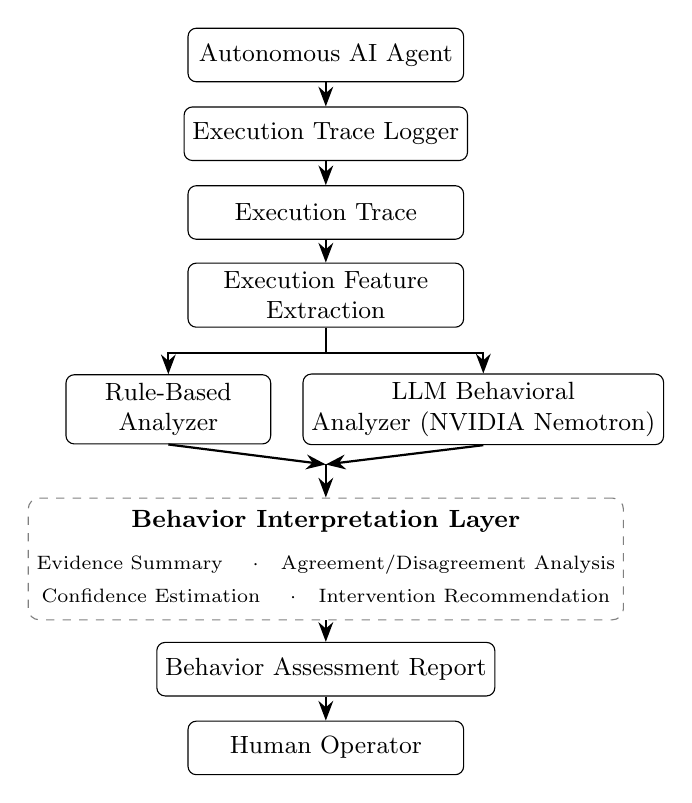
\begin{tikzpicture}[
  box/.style={draw, rounded corners=3pt, align=center,
              minimum height=0.68cm, font=\small, inner sep=3pt},
  arr/.style={-{Stealth[length=2.5mm]}, thick}
]

% Vertical pipeline
\node[box, minimum width=3.5cm] at (0,  0)    (agent)  {Autonomous AI Agent};
\node[box, minimum width=3.5cm] at (0, -1) (logger) {Execution Trace Logger};
\node[box, minimum width=3.5cm] at (0, -2)  (trace)  {Execution Trace};
\node[box, minimum width=3.5cm] at (0, -3.05) (feat)   {Execution Feature\\Extraction};

% Parallel analyzers
\node[box, minimum width=2.6cm] at (-2, -4.5) (rule) {Rule-Based\\Analyzer};
\node[box, minimum width=2.6cm] at (2, -4.5) (llm)  {LLM Behavioral\\Analyzer (NVIDIA Nemotron)};

\coordinate (merge) at (0, -5.2);

% Behavior interpretation layer
\node[box, minimum width=5.8cm, minimum height=1.45cm,
      draw=gray, dashed, rounded corners=4pt] at (0, -6.4) (interpret) {%
  \begin{tabular}{@{}c@{}}
    \textbf{\small Behavior Interpretation Layer}\\[4pt]
    {\scriptsize Evidence Summary \quad$\cdot$\quad Agreement/Disagreement Analysis}\\[1pt]
    {\scriptsize Confidence Estimation \quad$\cdot$\quad Intervention Recommendation}%
  \end{tabular}%
};

\node[box, minimum width=3.5cm] at (0, -7.8) (report) {Behavior Assessment Report};
\node[box, minimum width=3.5cm] at (0, -8.8) (human)  {Human Operator};

% Arrows
\draw[arr] (agent.south)   -- (logger.north);
\draw[arr] (logger.south)  -- (trace.north);
\draw[arr] (trace.south)   -- (feat.north);
\draw[arr] (feat.south)    -- ++(0,-0.32) -| (rule.north);
\draw[arr] (feat.south)    -- ++(0,-0.32) -| (llm.north);
\draw[arr] (rule.south)    -- (merge);
\draw[arr] (llm.south)     -- (merge);
\draw[arr] (merge)         -- (interpret.north);
\draw[arr] (interpret.south) -- (report.north);
\draw[arr] (report.south)  -- (human.north);

\end{tikzpicture}
\caption{LLMSheriff end-to-end pipeline. An autonomous agent produces an execution trace
that undergoes feature extraction and parallel analysis by a rule-based engine and an LLM
behavioral analyzer. The behavior interpretation layer aggregates their outputs---treating
agreement as a confidence signal and disagreement as diagnostic evidence---into a
structured behavior assessment report for a human operator.}
\label{fig:architecture}
\end{figure}

\subsection{Execution Feature Extraction}

Each trace event contains a timestamp, step label, action string, duration, and status.
After normalisation, eight features are computed: runtime, average latency, LLM call
count, tool call count, retry count, failure count, longest streak of repeated identical
actions, and a progress score (success rate penalised for repetition, capped at 1.0).

\subsection{Why a Hybrid Design?}

\textbf{Rule-based analyzer.} Rules are fast, deterministic, and fully explainable.
Thresholds can be inspected and modified without retraining. They perform well when
feature patterns are unambiguous---multiple failures, extreme repetition with low
progress, or clear recovery after errors.

\textbf{LLM-based analyzer.} Rules struggle on semantically ambiguous traces: polling
that resembles healthy execution, loops with moderate progress scores, or abandonment
without hard failures. The LLM behavioral analyzer receives the full trace and can
reason about action semantics, stage transitions, and whether observed activity plausibly
advances the goal. The trade-off is latency, API dependence, and less predictable
behaviour across prompts.

\textbf{Combining both.} Agreement suggests a higher-confidence classification.
Disagreement flags traces where features alone are insufficient---precisely the cases
where semantic reasoning may help and where human review is most valuable.

\subsection{State Vocabulary}

The prototype uses eight states: Planning, Executing, Waiting, Recovering, Stalled,
Abandoned, Completed, and Failed. The \emph{Recovering} state is central to the research
question: it represents an agent that encountered setbacks but adopted a new strategy
rather than abandoning the goal.

\subsection{Behavior Interpretation Layer}

Beyond state labels, the behavior interpretation layer produces:
\begin{itemize}
\item \textbf{Evidence summary}---positive and negative trace-derived indicators;
\item \textbf{Agreement/disagreement analysis}---when analyzers concur, agreement
strengthens confidence; when they differ, disagreement is surfaced as a diagnostic signal;
\item \textbf{Confidence estimation}---agreement-weighted confidence from both analyzers;
\item \textbf{Intervention recommendation}---no action, continue monitoring, or human
intervention suggested.
\end{itemize}

The aggregated output forms a \emph{behavior assessment report}. The prototype dashboard
visualises this report before it reaches a human operator.

% -----------------------------------------------------------------------
\section{Implementation}

The backend is implemented in FastAPI with SQLite persistence. The frontend is a Next.js dashboard that visualises the behavior assessment report:
dual predictions, metrics, an intent timeline, a behavior graph, evidence, disagreement
explanations, and intervention recommendations. Six preset scenarios and a step-by-step replay demo support
interactive exploration. The system runs via Docker Compose or local scripts.

The LLM behavioral analyzer calls NVIDIA Nemotron~\cite{nimotron} through a
chat-completions API with structured JSON output validation and heuristic fallback when
the API is unavailable.

% -----------------------------------------------------------------------
\section{Evaluation}

\subsection{Synthetic Corpus}

Because no public benchmark exists for agent intent-state labelling, we constructed a
reproducible synthetic corpus of 100 traces: 20 each for Completed, Recovering, Waiting,
Stalled, and Abandoned behaviour. Generators vary timestamps, action diversity, failure
counts, repetition streaks, and runtime while preserving class semantics. The generator
and evaluation scripts are included in the repository (\texttt{backend/scripts/}).

\subsection{Rule-Engine Results}

Table~\ref{tab:metrics} reports per-class precision, recall, and F1 for the rule-based
analyzer. Overall accuracy is 71\% with macro-F1 of 0.732.

\begin{table}[t]
\caption{Rule-engine performance on 100 synthetic traces}
\label{tab:metrics}
\centering
\small
\begin{tabular}{@{}lrrrr@{}}
\toprule
Class & Prec. & Recall & F1 & $n$ \\ \midrule
Completed & 1.00 & 1.00 & 1.00 & 20 \\
Recovering & 1.00 & 1.00 & 1.00 & 20 \\
Waiting & 0.00 & 0.00 & 0.00 & 20 \\
Stalled & 0.79 & 0.75 & 0.77 & 20 \\
Abandoned & 1.00 & 0.80 & 0.89 & 20 \\ \midrule
\textbf{Overall} & \multicolumn{3}{c}{Accuracy 0.71 / Macro-F1 0.732} & 100 \\ \bottomrule
\end{tabular}
\end{table}

\subsection{Confusion Patterns}

Table~\ref{tab:confusion} summarises the main confusion patterns. All 20 Waiting traces
were classified as Executing because polling behaviour is not encoded in the current
rule set. Five Stalled traces were classified as Executing when repetition did not reduce
the progress score below the stall threshold. Four Abandoned traces were classified as
Stalled when repetition dominated over runtime signals.

\begin{table}[t]
\caption{Selected confusion patterns (ground truth $\rightarrow$ prediction)}
\label{tab:confusion}
\centering
\small
\begin{tabular}{@{}lr@{}}
\toprule
Pattern & Count \\ \midrule
Waiting $\rightarrow$ Executing & 20 \\
Stalled $\rightarrow$ Executing & 5 \\
Abandoned $\rightarrow$ Stalled & 4 \\ \bottomrule
\end{tabular}
\end{table}

These errors motivate the LLM behavioral analyzer: they occur where semantics matter
more than thresholded statistics. A full LLM evaluation on the same corpus requires API
access and is left as ongoing work; the dual-analyzer dashboard is designed to surface
such cases interactively.

\subsection{Preset Scenario Validation}

Six hand-crafted dashboard scenarios (Healthy, Recovering, Looping, API Failure, Waiting,
Abandoned) provide qualitative validation and demonstration paths for reviewers. They
complement but do not replace the quantitative synthetic evaluation.

% -----------------------------------------------------------------------
\section{Limitations}

\begin{itemize}
\item Rule thresholds are hand-tuned, not optimised on labelled data.
\item The synthetic corpus approximates real agent behaviour but is not drawn from
production systems.
\item Waiting behaviour is not representable in the current rule vocabulary.
\item LLM evaluation at scale was not completed in this study due to API dependence.
\item No human inter-rater study has validated the state labels.
\end{itemize}

% -----------------------------------------------------------------------
\section{Conclusion}

LLMSheriff explores hybrid intent-state inference for autonomous AI agents. A rule engine
provides fast, explainable baselines; an LLM behavioral analyzer targets semantically
ambiguous traces; and a behavior interpretation layer treats agreement as confidence and
disagreement as diagnostic signal.
Evaluation on 100 synthetic traces shows strong performance on clear cases (Completed and
Recovering: F1 = 1.00) and systematic weakness on Waiting behaviour, supporting the
hybrid design motivation. Future work includes labelled real-world traces, calibrated
threshold learning, and large-scale LLM comparison.

% -----------------------------------------------------------------------
\begin{thebibliography}{00}

\bibitem{horkoff2016}
J.~Horkoff et al., ``Goal-oriented requirements engineering: An extended systematic
mapping study,'' \emph{Requirements Engineering}, vol.~21, no.~2, pp.~133--160, 2016.

\bibitem{dardenne1993}
A.~Dardenne, A.~van Lamsweerde, and S.~Fickas, ``Goal-directed requirements
acquisition,'' \emph{Science of Computer Programming}, vol.~20, nos.~1--2,
pp.~3--50, 1993.

\bibitem{carberry2001}
S.~Carberry, ``Techniques for plan recognition,'' \emph{User Modeling and User-Adapted
Interaction}, vol.~11, nos.~1--2, pp.~31--48, 2001.

\bibitem{leucker2009}
M.~Leucker and C.~Schallhart, ``A brief account of runtime verification,'' \emph{Journal
of Logic and Algebraic Programming}, vol.~78, no.~5, pp.~293--303, 2009.

\bibitem{otel}
OpenTelemetry Authors, ``OpenTelemetry specification v1.26,''
\url{https://opentelemetry.io/docs/specs/otel/}, 2024.

\bibitem{langsmith}
LangChain, ``LangSmith,'' \url{https://www.langchain.com/langsmith}, 2024.

\bibitem{langfuse}
Langfuse, ``Open-source LLM observability,'' \url{https://langfuse.com}, 2024.

\bibitem{nimotron}
NVIDIA, ``Nemotron-3-Ultra-550B,'' \url{https://build.nvidia.com/}, 2025.

\end{thebibliography}

\end{document}
